% Intended LaTeX compiler: xelatex
\documentclass[aspectratio=64,11pt]{beamer}
\usepackage{graphicx}
\usepackage{longtable}
\usepackage{wrapfig}
\usepackage{rotating}
\usepackage[normalem]{ulem}
\usepackage{amsmath}
\usepackage{amssymb}
\usepackage{capt-of}
\usepackage{hyperref}
\institute{Università di Siena}
\usepackage{localheader}
\usepackage{tikz}
\usepackage{booktabs,tabularx,tabularray}
\usepackage{setspace}
\usepackage{quoting}
\usepackage[italian]{babel}
\usepackage{fancybox}
\usepackage{tabularray}
\newcolumntype{R}{>{\raggedleft\arraybackslash}X}
\usetheme{default}
\author{Massimo D'Antoni}
\date{2023-2024}
\title{La tassazione dei beni e servizi}
\subtitle{Scienza delle Finanze}
\hypersetup{
 pdfauthor={Massimo D'Antoni},
 pdftitle={La tassazione dei beni e servizi},
 pdflang={Italian}}
\begin{document}

\maketitle


\section{Imposte sui beni e servizi}

%%%%%%%%%%%%%%%%%%%%%%%%%%%%%%%%%%%%%%%%%%%%
\begin{frame}{Classificazione}
\begin{center}
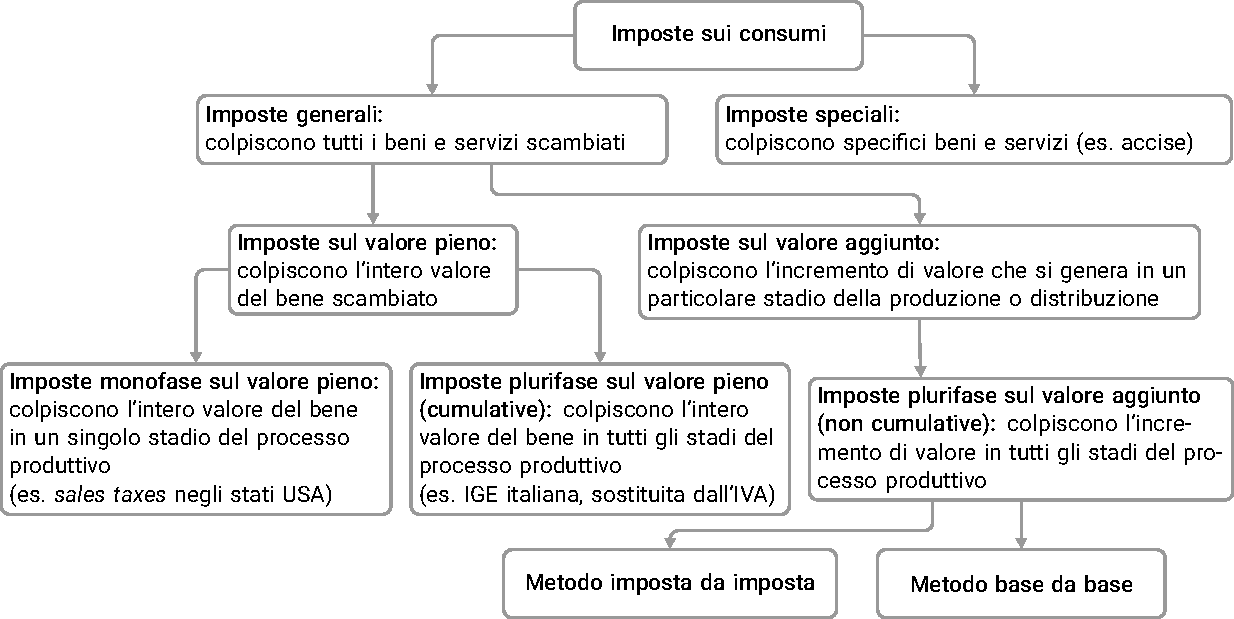
\includegraphics[width=\textwidth]{./figure/imposte-beni-servizi.pdf}
\end{center}
\end{frame}

%%%%%%%%%%%%%%%%%%%%%%%%%%%%%%%%%%%%%%%%%%%%
\begin{frame}{Evoluzione del gettito delle imposte sui beni e servizi}
\begin{center}
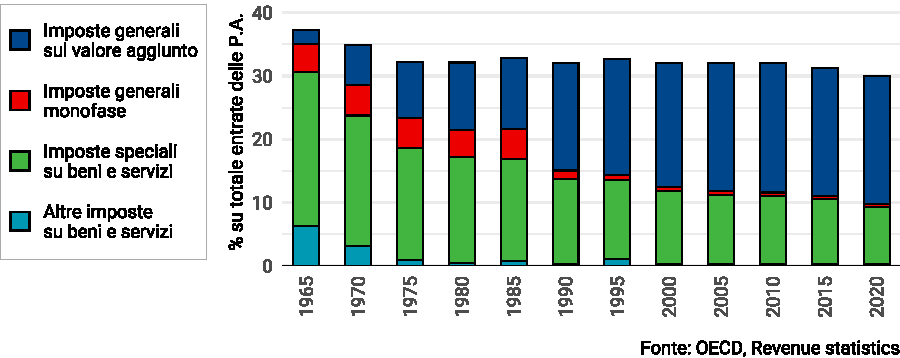
\includegraphics[width=\textwidth]{./figure/gettito-imposte-beni-OCSE-color.pdf}
\end{center}
\end{frame}

%%%%%%%%%%%%%%%%%%%%%%%%%%%%%%%%%%%%%%%%%%%%
\begin{frame}{Le imposte generali sul consumo: le varie fasi del processo produttivo}
\begin{itemize}
\item Le imposte possono gravare sulle diverse fasi del processo di produzione e
\end{itemize}
vendita. Ipotizziamo 3 fasi: produzione, ingrosso, dettaglio.

\begin{center}
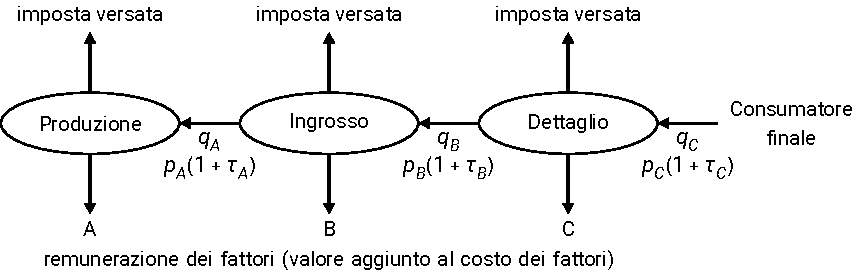
\includegraphics[width=\textwidth]{./figure/schema-imposte-generali.pdf}
\end{center}
\end{frame}

%%%%%%%%%%%%%%%%%%%%%%%%%%%%%%%%%%%%%%%%%%%%
\begin{frame}{Le imposte plurifase sul valore pieno}
\begin{itemize}
\item Nel caso di un'imposta sul valore pieno, i prezzi ai quali sono commisurate
le imposte (determinate su base netta) in ciascuna fase sono:
$$ p_A=A \qquad p_B=B+q_A \qquad p_C=C+q_C $$
\item Visto che $q_i=(1+\tau_i)p_i$, procedendo per sostituzioni successive:
\begin{equation*}
\begin{split}
  \tau_Ap_A&= \tau_AA \\
  \tau_Bp_B&= \tau_B(B + q_A) = \tau_B\big[B+ (1+t_A)A\big] \\
  \tau_Cp_C&= \tau_C(C + q_B) = \tau_C\Big[C+(1+\tau_B)\big[B+ (1+t_A)A\big]\Big].
\end{split}
\end{equation*}
da cui calcoliamo l'imposta totale:
\begin{equation*}
T^{PC} = \tau_CC + \Big[\tau_B+\tau_C(1+\tau_B)\Big]B
+ \Big[\tau_A + \tau_B(1+\tau_A) + \tau_C(1+\tau_B)(1+\tau_A)\Big]A 
\end{equation*}
\item Con $\tau$ uniforme si evidenzia il carattere «cumulativo» dell'imposta:
\begin{equation*}
T^{PC}=\tau\, C + \tau\,\big[2+\tau\big]\, B + \tau\,\big[3 + \tau(3+\tau)\big]\, A.
\end{equation*}
\end{itemize}
\end{frame}

%%%%%%%%%%%%%%%%%%%%%%%%%%%%%%%%%%%%%%%%%%%%
\begin{frame}{Le imposte plurifase sul valore pieno: l'incentivo all'integrazione verticale}
\begin{itemize}
\item Nell'ipotesi $A=B=C=100$ e $\tau=10\%$ (uniforme):
\begin{center}
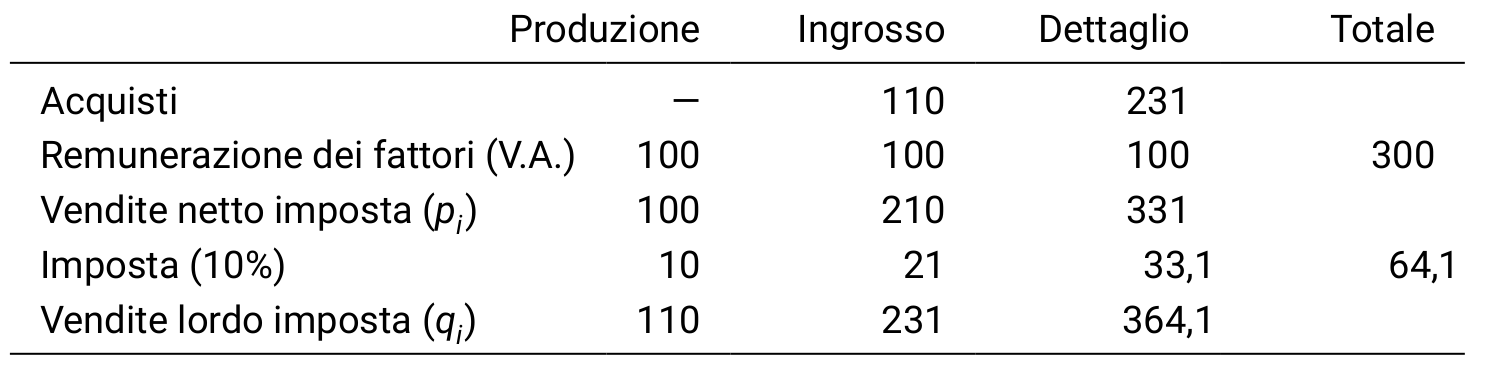
\includegraphics[width=.8\textwidth]{./figure/imposte-plurifase-esempio-1.png}
\end{center}
L'aliquota effettiva su base netta è: $64,1/300=21,36\%$

\item Se c'è integrazione verticale di Produzione e Ingrosso:
\begin{center}
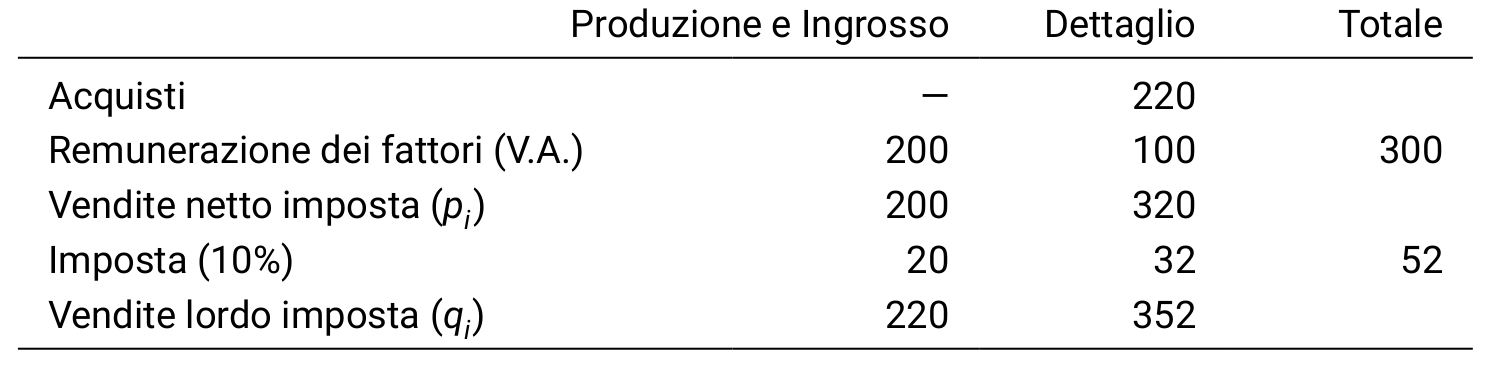
\includegraphics[width=.8\textwidth]{./figure/imposte-plurifase-esempio-2.png}
\end{center}
L'aliquota effettiva su base netta è: $52/300=17,3\%$
\end{itemize}
\end{frame}

%%%%%%%%%%%%%%%%%%%%%%%%%%%%%%%%%%%%%%%%%%%%
\begin{frame}{L'imposta monofase}
\begin{itemize}
\item Per evitare gli inconvenienti di un'imposta cumulativa possiamo applicare
l'imposta sul valore pieno una sola volta, in uno dei tre stadi:
\begin{itemize}
\item cessione al grossista: $\tau A$
\item cessione al dettagliante: $\tau(A+B)$
\item cessione al consumatore finale: $\tau(A+B+C)$
\end{itemize}
\item Nel caso di cessione al consumatore finale l'aliquota effettiva è $\tau$,
negli altri casi è inferiore. Ad esempio, nel caso in cui ad essere tassata
sia la cessione al dettagliante, l'aliquota effettiva è:
$$ \frac{\tau(A+B)}{A+B+C}<\tau $$
\item Un esempio di monofase: le \emph{sales taxes} americane, applicate dai singoli
stati nella fase di vendita al dettaglio.
\end{itemize}
\end{frame}

%%%%%%%%%%%%%%%%%%%%%%%%%%%%%%%%%%%%%%%%%%%%
\begin{frame}{L'imposta sul valore aggiunto}
\begin{itemize}
\item Colpisce in ciascuna fase l'\alert{incremento} di valore del bene scambiato.
\end{itemize}

\begin{figure}[htbp]
\centering
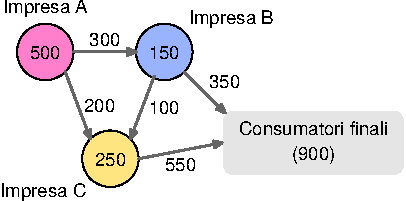
\includegraphics[width=10cm]{./figure/flussi-VA-metaflow-1.pdf}
\end{figure}

\begin{itemize}
\item La somma del valore aggiunto delle imprese è pari al consumo finale, a sua
volta pari al fatturato totale meno gli acquisti di beni intermedi (le
transazioni tra imprese).
\end{itemize}
\end{frame}

%%%%%%%%%%%%%%%%%%%%%%%%%%%%%%%%%%%%%%%%%%%%
\begin{frame}{L'imposta sul valore aggiunto: metodi di calcolo}
Due metodi per la determinazione della base imponibile:
\begin{itemize}
\item \textbf{Base da base (\emph{subtraction method})}.
\begin{itemize}
\item L'imposta non si applica alle singole transazioni, ma al valore aggiunto
complessivo (differenza tra totale vendite e totale acquisti) dei soggetti
che effettuano vendite di beni e servizi.
\item L'imposta appare formalmente simile a un'imposta diretta, applicata alla
remunerazione complessiva dei fattori.
\item L'aliquota è definita \alert{su base lorda}.
\end{itemize}

\item \textbf{Imposta da imposta (\emph{invoice credit method})}.
\begin{itemize}
\item L'imposta è calcolata su ogni singola transazione. In fattura sono
indicati prezzo netto, imposta e prezzo lordo.
\item Formalmente è a carico dell'acquirente, ma viene versata dal venditore che
l'ha incassata.
\item L'aliquota è definita \alert{su base netta}.
\end{itemize}
\end{itemize}
\end{frame}

%%%%%%%%%%%%%%%%%%%%%%%%%%%%%%%%%%%%%%%%%%%%
\begin{frame}{L'imposta sul valore aggiunto col metodo base da base}
\begin{itemize}
\item Calcoliamo l'imposta (indicando con $t$ le aliquote su base lorda):
\begin{equation*}
T^{BB} = t_Aq_A + t_B(q_B-q_A) + t_C(q_C-q_B).
\end{equation*}
\item Visto che:
\begin{equation*}
A=(1-t_A)q_A\qquad B=(1-t_B)(q_B-q_A)\qquad C=(1-t_C)(q_C-q_B)
\end{equation*}
possiamo scrivere:
\begin{equation*}
  T^{BB} = \frac{t_A}{1-t_A}A + \frac{t_B}{1-t_B}B +\frac{t_C}{1-t_C}C.
\end{equation*}
formula che evidenzia l'assenza di effetti «cumulativi».
\item Inoltre, se $t$ è uniforme le formule si semplificano:
\begin{equation*}
  T^{BB} = t\,q_C = \frac{t}{1-t}(A + B+ C).
\end{equation*}
per cui l'aliquota effettiva è $t/(1-t)$, aliquota \emph{su base netta}
corrispondente all'aliquota legale \emph{su base lorda} $t$.
\end{itemize}
\end{frame}

%%%%%%%%%%%%%%%%%%%%%%%%%%%%%%%%%%%%%%%%%%%%
\begin{frame}{L'imposta sul valore aggiunto col metodo base da base: esempio}
  \vspace*{-3.5mm}\footnotesize
  \begin{block}{}
    \textbf{Aliquota uniforme:} 20\%\\
    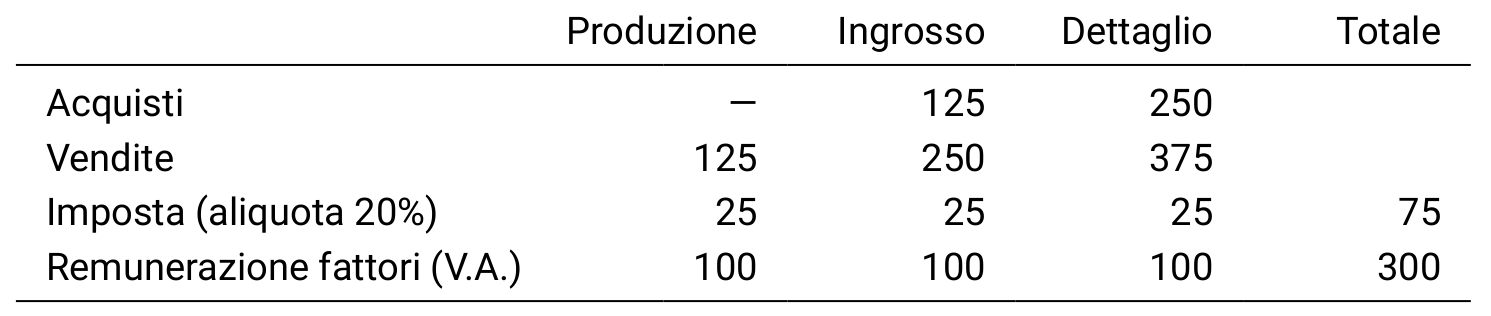
\includegraphics[width=.8\textwidth]{./figure/esempio-base-da-base-aliquota-uniforme.png}\\
    L'imposta complessiva è 75€, dunque l'aliquota effettiva su base lorda
    è $75/375=20\%$, quella su base netta è $75/300=25\%$.
  \end{block}
  \begin{block}{}
    \textbf{Aliquota differenziata:} 20\% nelle fasi di produzione e ingrosso, 10\% al
      dettaglio\\
      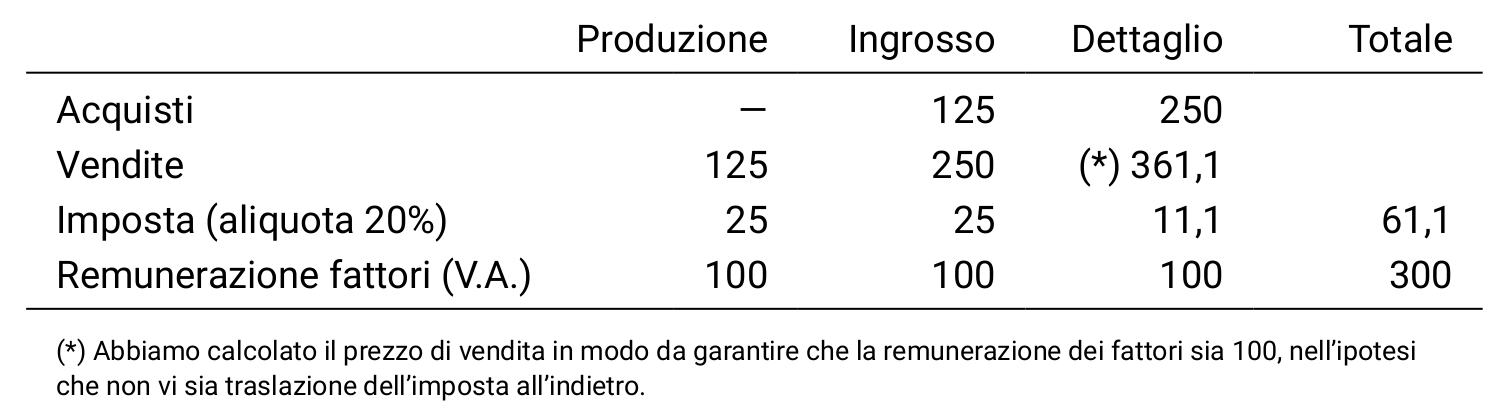
\includegraphics[width=.8\textwidth]{./figure/esempio-base-da-base-aliquota-differenziata.png}\\
    L'imposta complessiva è 61,1€, l'aliquota effettiva su base \emph{lorda} è
    61,1/361,1=16,92\%, maggiore dell'aliquota pagata dal consumatore
    finale. L'aliquota effettiva su base netta è 61,1/361,1=20,36\%.
  \end{block}
\end{frame}


%%%%%%%%%%%%%%%%%%%%%%%%%%%%%%%%%%%%%%%%%%%%
\begin{frame}{L'imposta sul valore aggiunto col metodo imposta da imposta}
\begin{itemize}
\item Indichiamo con $\tau_A$, $\tau_B$ e $\tau_C$ le aliquote, su base netta,
applicate nelle tre fasi al prezzo al netto dell'imposta.
\item Le imposte versate sono:
\begin{equation*}
\tau_Ap_A \qquad \tau_Bp_B-\tau_Ap_A \qquad \tau_Cp_C-\tau_Bp_B
\end{equation*}
per cui:
\begin{equation*}
  T^{II}=\tau_Ap_A + (\tau_Bp_B-\tau_Ap_A) +
  (\tau_C p_C-\tau_Bp_B)=\tau_Cp_C.
\end{equation*}
\item Il valore aggiunto al costo dei fattori è:
\begin{equation*}
A=p_A \qquad B = p_B-p_A \qquad C=p_C-p_B
\end{equation*}
dunque:
\begin{equation*}
\begin{split}
  T^{II}&=\tau_AA + [\tau_B(A+B)-\tau_AA] + [\tau_C(A+B+C)-\tau_B(A+B)]\\
  &=\tau_C(A+B+C).
\end{split}
\end{equation*}
\item L'imposta effettiva coincide con l'aliquota applicata al consumatore finale.
\end{itemize}
\end{frame}

%%%%%%%%%%%%%%%%%%%%%%%%%%%%%%%%%%%%%%%%%%%%
\begin{frame}{L'imposta sul valore aggiunto col metodo imposta da imposta: esempio}
\begin{block}{}
\textbf{Con aliquota uniforme} $\tau=25\%$\\(corrispondente a un'aliquota su base
lorda del 20\%):\\
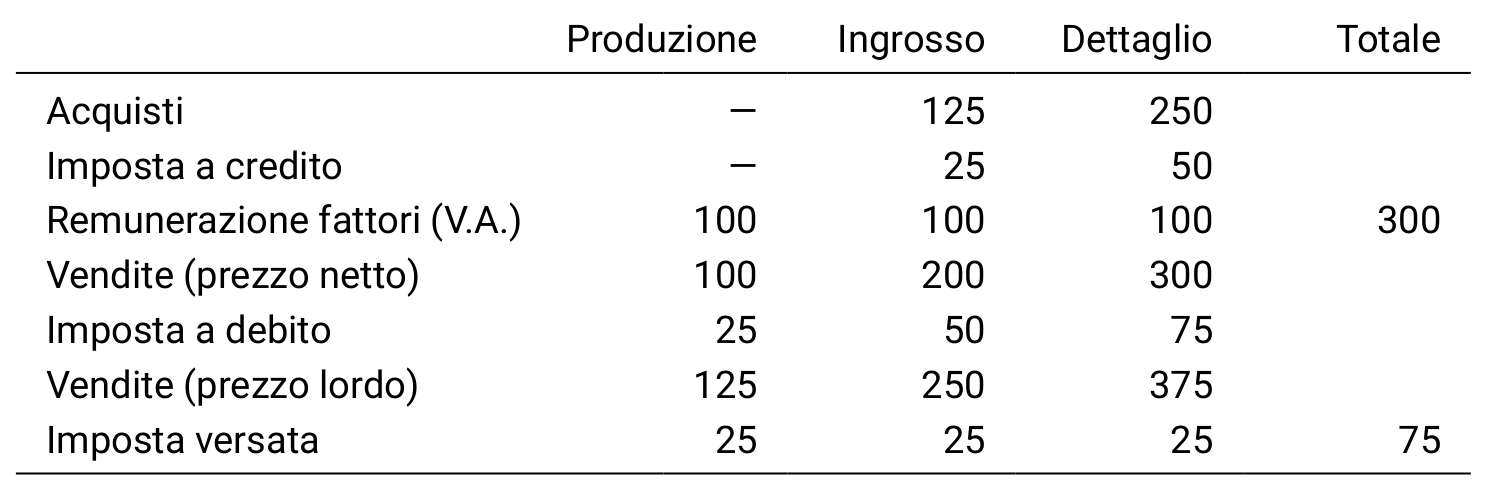
\includegraphics[width=\textwidth]{./figure/esempio-imposta-da-imposta-1.png}\\
L'imposta complessiva è 75€, l'aliquota effettiva è: $75/300=25\%$,
esattamente come nel precedente esempio di applicazione del metodo base da
base
\end{block}
\end{frame}


%%%%%%%%%%%%%%%%%%%%%%%%%%%%%%%%%%%%%%%%%%%%
\begin{frame}{L'imposta sul valore aggiunto col metodo imposta da imposta: esempio}
\begin{block}{}
\textbf{Con aliquota differenziata} $\tau_A=\tau_B=25\%$ e $\tau_C=11,1\%$\\
(quest'ultima corrisponde a un'aliquota su base lorda del 10\%)\\
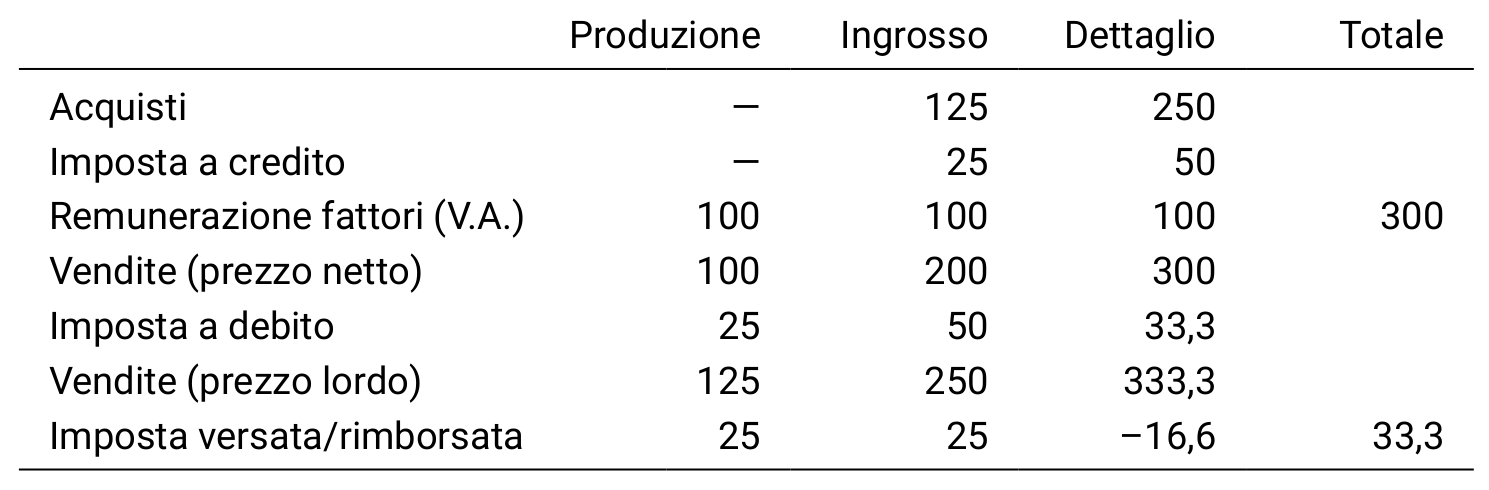
\includegraphics[width=\textwidth]{./figure/esempio-imposta-da-imposta-2.png}\\
Il dettagliante ha diritto al rimborso dell'IVA pagata al grossista in
eccesso sull'IVA a debito.

L'imposta complessiva è 33,3€, l'aliquota effettiva è: $33,3/300=11,1\%$.
\end{block}
\end{frame}

%%%%%%%%%%%%%%%%%%%%%%%%%%%%%%%%%%%%%%%%%%%%
\begin{frame}{Vantaggi e svantaggi del metodo imposta da imposta}
\begin{itemize}
\item Il metodo imposta da imposta presenta diversi vantaggi: trasparenza e
neutralità rispetto all'integrazione verticale anche in presenza di aliquote
differenziate tra le varie fasi.
\item Esso pone tuttavia anche qualche problema in alcuni casi:
\begin{enumerate}
\item \alert{beni rimessi in commercio dopo l'uso}: se un privato vende l'auto
all'officina, che la rivende applicando l'IVA\ldots{}.
\item \alert{servizi resi dal settore finanziario e assicurativo}: difficile
determinare il valore del servizio, remunerato con il margine tra
interessi attivi e passivi;
\item \alert{servizi della Pubblica amministrazione}, forniti gratuitamente o ad un
prezzo inferiore al costo.
\end{enumerate}
\item Nel caso 1 la base imponibile è la differenza tra prezzo di vendita e prezzo
di acquisto dell'auto dal privato («metodo del margine»)
\item Nei casi 2 e 3 la soluzione è l'\alert{esenzione}. Attenzione: c'è differenza tra
operazioni esenti e operazioni non imponibili.
\end{itemize}
\end{frame}

%%%%%%%%%%%%%%%%%%%%%%%%%%%%%%%%%%%%%%%%%%%%
\begin{frame}{Operazioni imponibili IVA: esempio}
\begin{itemize}
\item Su un'operazione non imponibile l'effetto è quello che ci sarebbe con
aliquota IVA pari a zero. Questo perché al venditore, che non applica l'IVA
all'acquirente, viene riconosciuto il credito per l'IVA sugli acquisti.
\item Se è non imponibile una vendita a un consumatore finale (B2C, \emph{business-to-consumer}):
\end{itemize}

\begin{center}
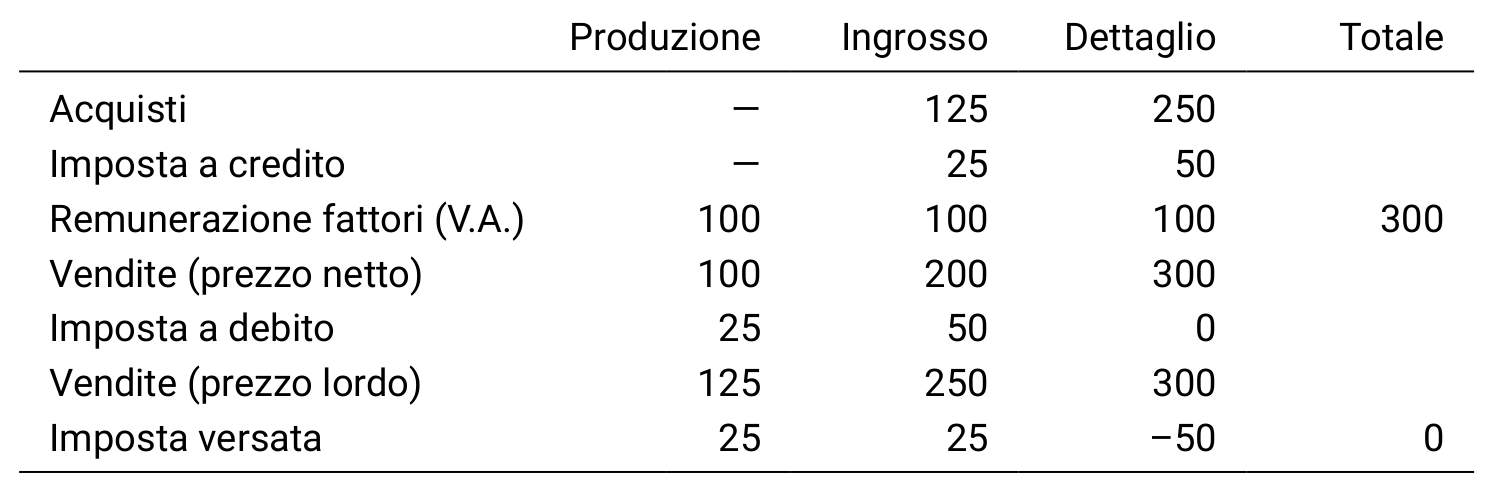
\includegraphics[width=\textwidth]{./figure/esempio-non-imponibile-IVA-B2C.png}
\end{center}
\end{frame}


%%%%%%%%%%%%%%%%%%%%%%%%%%%%%%%%%%%%%%%%%%%%
\begin{frame}{Operazioni imponibili IVA: esempio /2}
\begin{itemize}
\item Se è non imponibile una vendita a un altro soggetto IVA (B2B,
\emph{business-to-business}), ad es. dal grossista al dettagliante:
\end{itemize}

\begin{center}
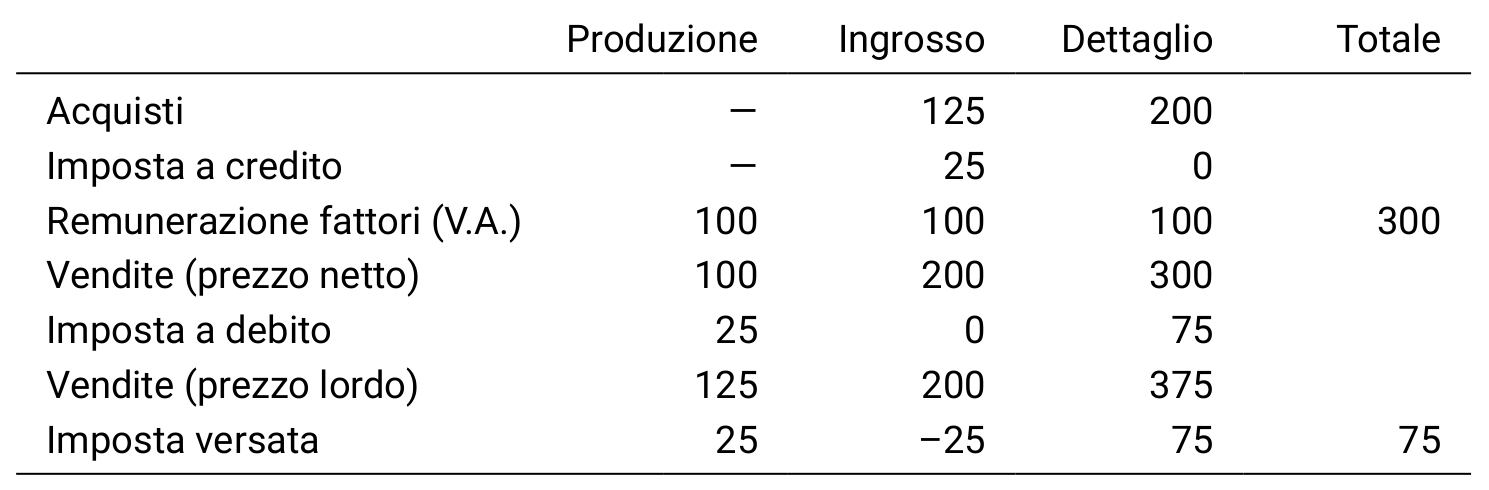
\includegraphics[width=\textwidth]{./figure/esempio-non-imponibile-IVA-B2B.png}
\end{center}

\begin{itemize}
\item In questo caso la non imponibilità dell'operazione non ha alcun effetto sul
prezzo e sull'imposta finale pagati. L'aliquota effettiva coincide con
l'aliquota legale per il consumatore.
\end{itemize}
\end{frame}

%%%%%%%%%%%%%%%%%%%%%%%%%%%%%%%%%%%%%%%%%%%%
\begin{frame}{Operazioni esenti IVA: esempio}
\begin{itemize}
\item In un'operazione esente chi vende non ha diritto all'IVA a credito sugli
acquisti: il prezzo del bene resta dunque gravato dell'IVA pagata «a monte»
\item Se operazione B2C (\emph{business-to-consumer}) l'imposta esclude il valore
aggiunto $C$: $T^{II}=\tau_A A + [\tau_B(A+B)-\tau_A A] = \tau_B (A+B)$.
\end{itemize}

\begin{center}
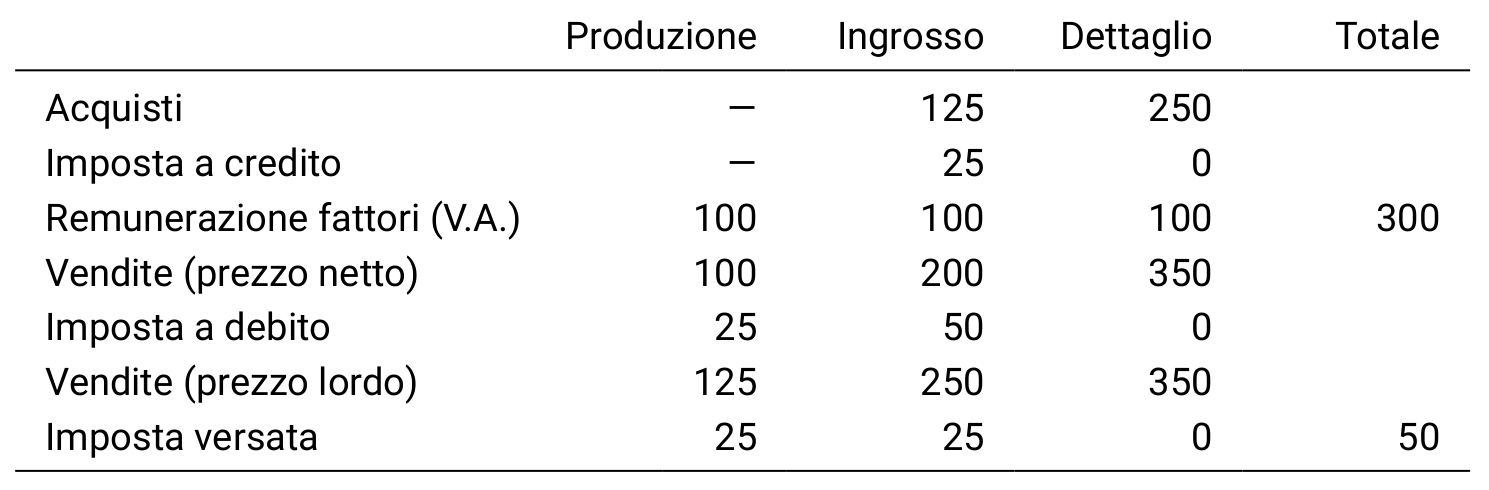
\includegraphics[width=\textwidth]{./figure/esempio-esente-IVA-B2C.png}
\end{center}
\end{frame}



%%%%%%%%%%%%%%%%%%%%%%%%%%%%%%%%%%%%%%%%%%%%
\begin{frame}{Operazioni esenti IVA: esempio /2}
\begin{itemize}
\item Se operazione B2B (\emph{business-to-business}), ad es. cessione al dettagliante, abbiamo:
$T^{II}=\tau_A A + \tau_C(A+B+C)$, con l'effetto di tassare due volte $A$.
\end{itemize}

\begin{center}
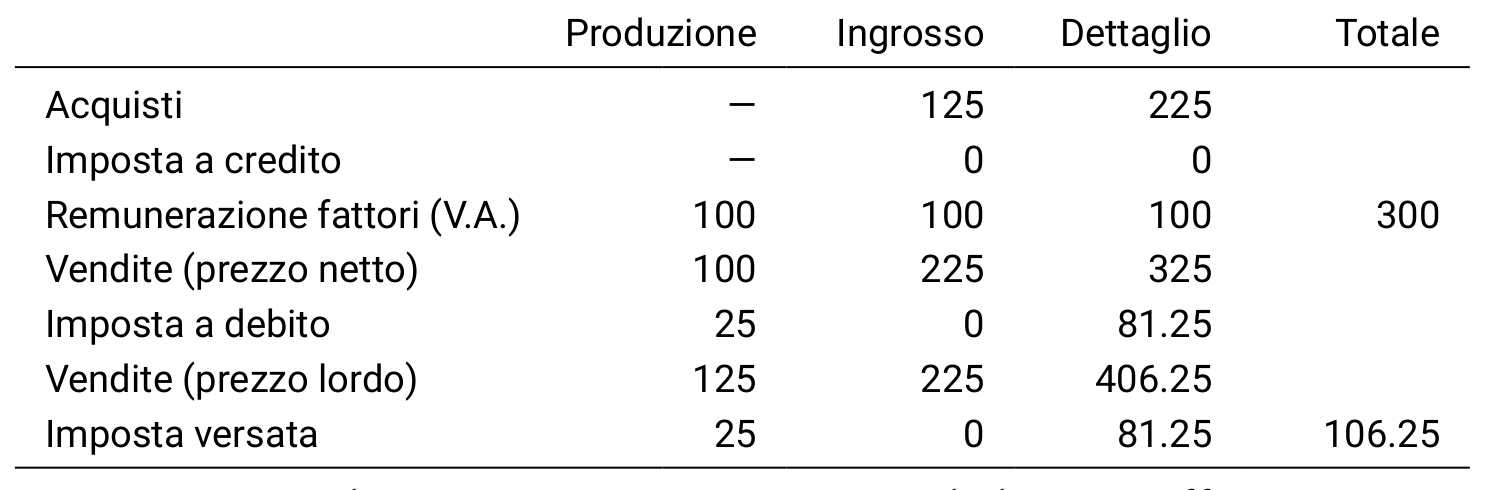
\includegraphics[width=\textwidth]{./figure/esempio-esente-IVA-B2B.png}
\end{center}
\end{frame}


\section{L'IVA in Italia e in Europa}



%%%%%%%%%%%%%%%%%%%%%%%%%%%%%%%%%%%%%%%%%%%%
\begin{frame}{L'IVA in Italia}
\begin{itemize}
\item Introdotta nel 1973. In precedenza era presenta l'IGE (Imposta Generale
sulle Entrate), un'imposta plurifase sul valore pieno.
\item Il suo \emph{presupposto} è una delle seguenti circostanze:
\begin{itemize}
\item la cessione di beni nel territorio dello stato
\item la prestazione di servizi da parte di soggetti residenti se effettuati
nell'esercizio di imprese o di arti e professioni;
\item gli acquisti intracomunitari e le importazioni, da chiunque effettuati.
\item l'autoconsumo (nell'esercizio di impresa o arti e professioni)
\end{itemize}
Nota bene: il riferimento alla cessione fa sì che l'imposta sia «su base
finanziaria» e non «su base reale» (non sono tassate scorte e rimanenze).

\item \emph{Soggetti passivi} sono gli imprenditori, gli esercenti arti o professioni,
i soggetti che effettuano importazioni o acquisti intracomunitari. I
soggetti IVA sono tenuti a versare l'imposta con \alert{obbligo di rivalsa} sugli
acquirenti.

\item La \emph{base imponibile} è l'ammontare complessivo del corrispettivo per
l'acquisto del bene o del servizio, cui l'aliquota si applica \alert{su base netta}.
\end{itemize}
\end{frame}

%%%%%%%%%%%%%%%%%%%%%%%%%%%%%%%%%%%%%%%%%%%%
\begin{frame}{Aliquote Iva in Italia}
\begin{itemize}
\item Le \emph{aliquote}, la cui determinazione è soggetta a vincoli comunitari,
sono:
\begin{itemize}
\item aliquota \alert{normale} 22\% (era al 20\% fino al 2011)
\item aliquota \alert{ridotta} 10\% (es. carne, pesce, zucchero\dots{}, hotel e
ristoranti, ristrutturazioni edilizie, acqua, farmaceutici, trasporti,
cinema e teatri, gas naturale ed elettricità)
\item aliquota \alert{ridotta} 5\% per prestazioni rese da cooperative sociali
\item aliquota \alert{super-ridotta} 4\% (es. pasta, pane, burro, dispositivi medici
per disabili, libri e periodici, alcune ristrutturazioni---ma anche
licenze TV)
\end{itemize}
\item Sono \alert{esenti} (aliquota zero):
\begin{itemize}
\item servizi di credito e assicurazioni;
\item servizi sanitari, servizi educativi, servizi pubblici di trasporto, alcuni
servizi culturali;
\item i servizi resi da imprese e lavoratori autonomi assoggettati al regime
sostitutivo (ricavi non superiori a 65 mila euro).
\end{itemize}

\item La presenza di aliquote ridotte su beni essenziali determina un (limitato)
effetto di progressività.
\end{itemize}
\end{frame}

%%%%%%%%%%%%%%%%%%%%%%%%%%%%%%%%%%%%%%%%%%%%
\begin{frame}{Aliquote Iva in Europa (2023)}
\begin{columns}
\begin{column}{.5\columnwidth}
\scriptsize
\begin{tabular}{p{1.5cm}ccc}
  \toprule
& ordinaria & ridotta & \parbox{1cm}{\centering super ridotta} \\ 
\midrule
Austria & 20 & 10 / 13 &  \\ 
Belgio & 21 & 6 / 12 &  \\ 
Bulgaria & 20 & 9 &  \\ 
Cipro & 19 & 5 / 9 &  \\ 
Croazia & 25 & 5 / 13 &  \\ 
Danimarca & 25 &  &  \\ 
Estonia & 20 & 9 &  \\ 
Finlandia & 24 & 10 /14 &  \\ 
Francia & 20 & 5,5 / 10 & 2,1 \\ 
Germania & 19 & 7 &  \\ 
Grecia & 24 & 6 / 13 &  \\ 
Irlanda & 23 & 9 / 13,5 & 4,8 \\ 
Italia & 22 & 5 / 10 & 4 \\ 
Lettonia & 21 & 5 / 12 &  \\ 
\bottomrule
\end{tabular}
\end{column}

\begin{column}{.5\columnwidth}
\scriptsize
\begin{tabular}{p{1.5cm}ccc}
  \toprule
& ordinaria & ridotta & \parbox{1cm}{\centering super ridotta} \\ 
\midrule
Lituania & 21 & 5 / 9 &  \\ 
Lussemburgo & 17 & 8 & 3 \\ 
Malta & 18 & 5 / 7 &  \\ 
Paesi Bassi & 21 & 9 &  \\ 
Polonia & 23 & 5 / 8 &  \\ 
Portogallo & 23 & 6 / 13 &  \\ 
Regno Unito & 20 & 5 &  \\ 
Rep. Ceca & 21 & 10 / 15 &  \\ 
Romania & 19 & 5 / 9 &  \\ 
Slovacchia & 20 & 10 &  \\ 
Slovenia & 22 & 5 / 9.5 &  \\ 
Spagna & 21 & 10 & 4 \\ 
Svezia & 25 & 6 / 12 &  \\ 
Ungheria & 27 & 5 / 18 &  \\ 
\bottomrule
\end{tabular}
\end{column}
\end{columns}

\footnotesize
\begin{itemize}
\item Entro il quadro definito dalla normativa europea i paesi UE hanno la
possibilità di fissare le proprie aliquote
\item Le aliquote ridotte sono applicabili solo a categorie esplicitamente
previste da normativa europea (Annex III della Direttiva sull'Iva
2006/112/EC).
\end{itemize}

→ \href{https://ec.europa.eu/taxation\_customs/sites/taxation/files/resources/documents/taxation/vat/how\_vat\_works/rates/vat\_rates\_en.pdf}{VAT Rates Applied in the Member States of the European Union} 
\end{frame}



%%%%%%%%%%%%%%%%%%%%%%%%%%%%%%%%%%%%%%%%%%%%
\begin{frame}{Aliquote Iva in Italia: evoluzione}
\begin{center}
\centering
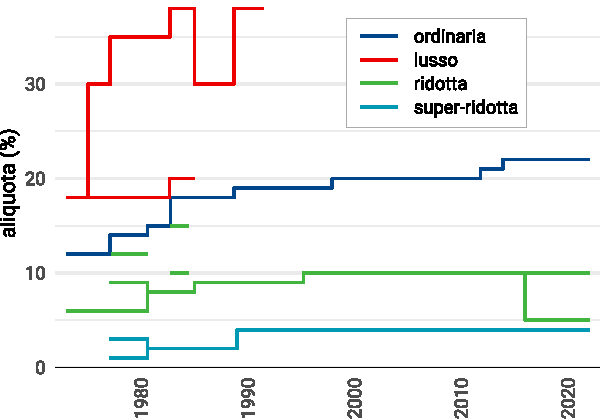
\includegraphics[height=7cm]{./figure/IVA-aliquote-Italia-color.pdf}
\end{center}
\end{frame}


%%%%%%%%%%%%%%%%%%%%%%%%%%%%%%%%%%%%%%%%%%%%
\begin{frame}{Quali sono i vantaggi dell'IVA?}
\begin{itemize}
\item A differenza di altre imposte generali sugli scambi, l'IVA è \alert{neutrale} e
\alert{trasparente}:
\begin{itemize}
\item non rende conveniente l'integrazione verticale;
\item non influisce sulle scelte degli input.
\end{itemize}
Diamond e Mirrlees (1971): se i mercati sono concorrenziali non è mai
efficiente distorcere i prezzi alla produzione, quale che sia l'obiettivo
redistributivo che si vuole perseguire.
\item Difficoltà di evasione: la determinazione dell'imposta è il risultato di
molteplici operazioni di compravendita, in cui c'è contrasto di interessi
tra le parti. Tuttavia:
\begin{itemize}
\item interesse del consumatore finale a evadere;
\item l'evasione in una fase può sollecitare l'evasione nella fase precedente;
\item il rimborso dell'IVA può essere occasione per frodi fiscali (ad es. la
«frode carosello»).
\end{itemize}
\end{itemize}
\end{frame}

%%%%%%%%%%%%%%%%%%%%%%%%%%%%%%%%%%%%%%%%%%%%
\begin{frame}{L'evasione dell'IVA}
\begin{itemize}
\item L'evasione dell'IVA non è inferiore a quella delle altre imposte
\end{itemize}

\begin{center}
\centering
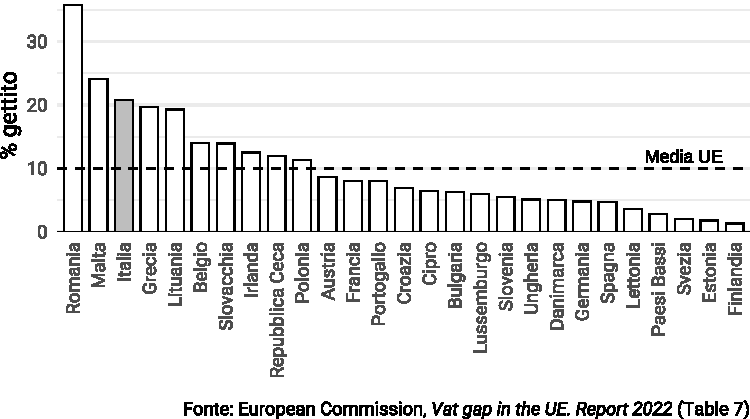
\includegraphics[height=5cm]{./figure/IVA-tax-gap.pdf}
\end{center}

\begin{itemize}
\item Alcune soluzioni introdotte negli ultimi anni:
\begin{itemize}
\item il \emph{reverse charge};
\item lo \emph{split payment} («scissione dei pagamenti»).
\end{itemize}
\end{itemize}
\end{frame}

%%%%%%%%%%%%%%%%%%%%%%%%%%%%%%%%%%%%%%%%%%%%
\begin{frame}{\emph{Reverse charge}}
\begin{itemize}
\item Con il \emph{reverse charge} (inversione contabile), il versamento non viene
effettuato dal venditore ma dall'acquirente, che contabilizza l'Iva sugli
acquisti sia a debito che a credito (analogamente a quanto accade per le
operazioni intracomunitarie)
\item Lo scopo è scoraggiare l'evasione dell'Iva realizzata nelle fasi intermedie
es. attraverso false fatturazioni per aumentare l'Iva a credito
\item Giudicata efficace, ma
\begin{itemize}
\item modifica in modo rilevante il funzionamento dell'Iva (richiede accordo con
UE)
\item può incentivare evasione nella fase finale, e dunque va accompagnata dal
potenziamento dell'attività di contrasto in tale fase
\end{itemize}
\end{itemize}
\end{frame}


\section{Le imposte speciali sui beni e servizi}


%%%%%%%%%%%%%%%%%%%%%%%%%%%%%%%%%%%%%%%%%%%%
\begin{frame}{Imposte indirette: classificazione amministrativa e gettito (2018)}
  \begin{columns}
    \begin{column}{.7\columnwidth}
      \begin{figure}[htbp]
        \vspace*{-5mm}
        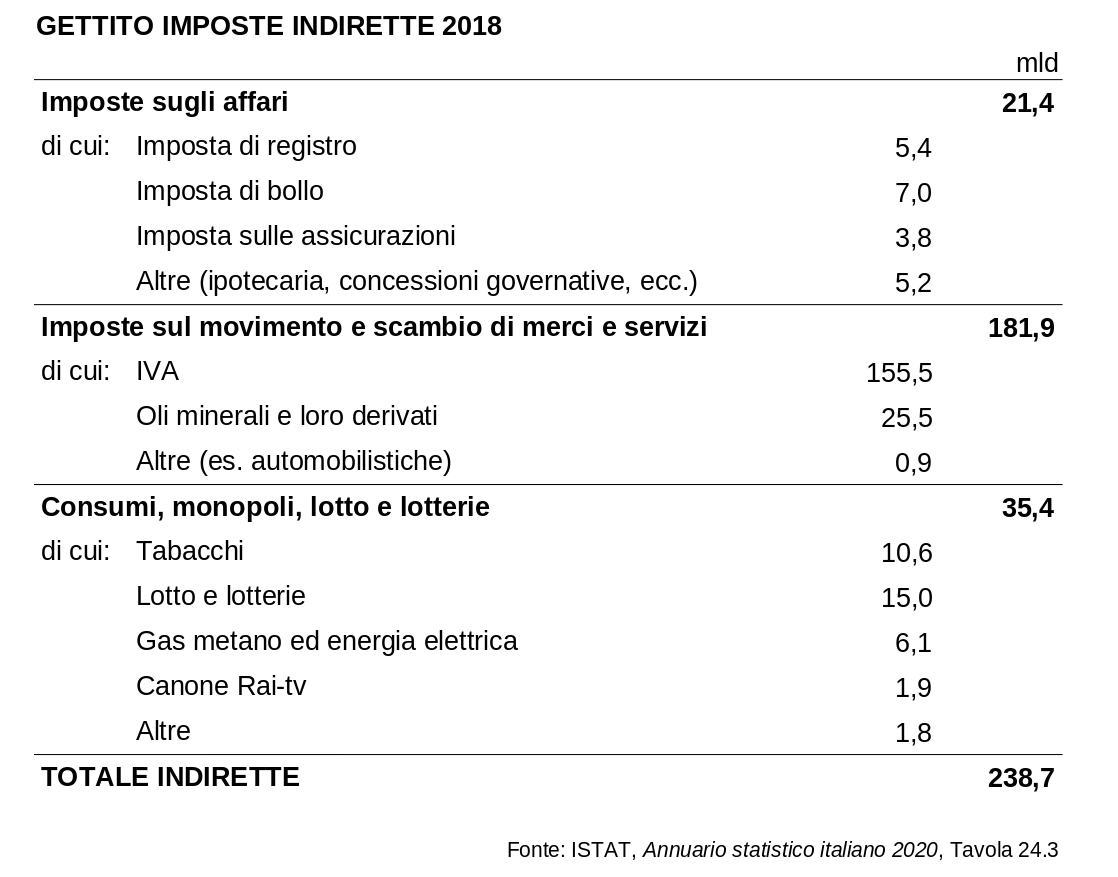
\includegraphics[height=7cm]{./figure/imposte-indirette-2018.png}
      \end{figure}
    \end{column}
    \begin{column}{.3\columnwidth}
      Si tratta di un insieme molto eterogeneo di imposte.
      \bigskip

      Alcune di esse sono anacronistiche, hanno elevati costi amministrativi e un
      gettito limitato.
    \end{column}
  \end{columns}
\end{frame}

%%%%%%%%%%%%%%%%%%%%%%%%%%%%%%%%%%%%%%%%%%%%
\begin{frame}{Imposte speciali}
\begin{itemize}
\item Il ruolo delle imposte \alert{speciali} (= applicate a particolari categorie di
beni di consumo) è andato diminuendo nel tempo.
\item Tuttavia, restano alcune \alert{accise} (= imposte speciali e nella maggior parte
dei casi specifiche) che mantengono una certa importanza, in quanto
colpiscono beni il cui consumo lo Stato desidera scoraggiare («sin taxes»):
\begin{itemize}
\item accisa sul tabacco;
\item accisa sulle bevande alcoliche;
\item accisa sui combustibili fossili;
\item accisa sull'energia elettica.
\end{itemize}
In alcuni paesi:
\begin{itemize}
\item imposte sulle bevande zuccherate e sui cibi contenenti grassi.
\end{itemize}
\item Assimilabile alla «sin tax» è anche l'imposizione sui giochi (lotterie,
scommesse, \emph{slot machine}, giochi d'azzardo on-line)
\end{itemize}
\end{frame}

%%%%%%%%%%%%%%%%%%%%%%%%%%%%%%%%%%%%%%%%%%%%
\begin{frame}{Imposte speciali: il gettito}
\begin{center}
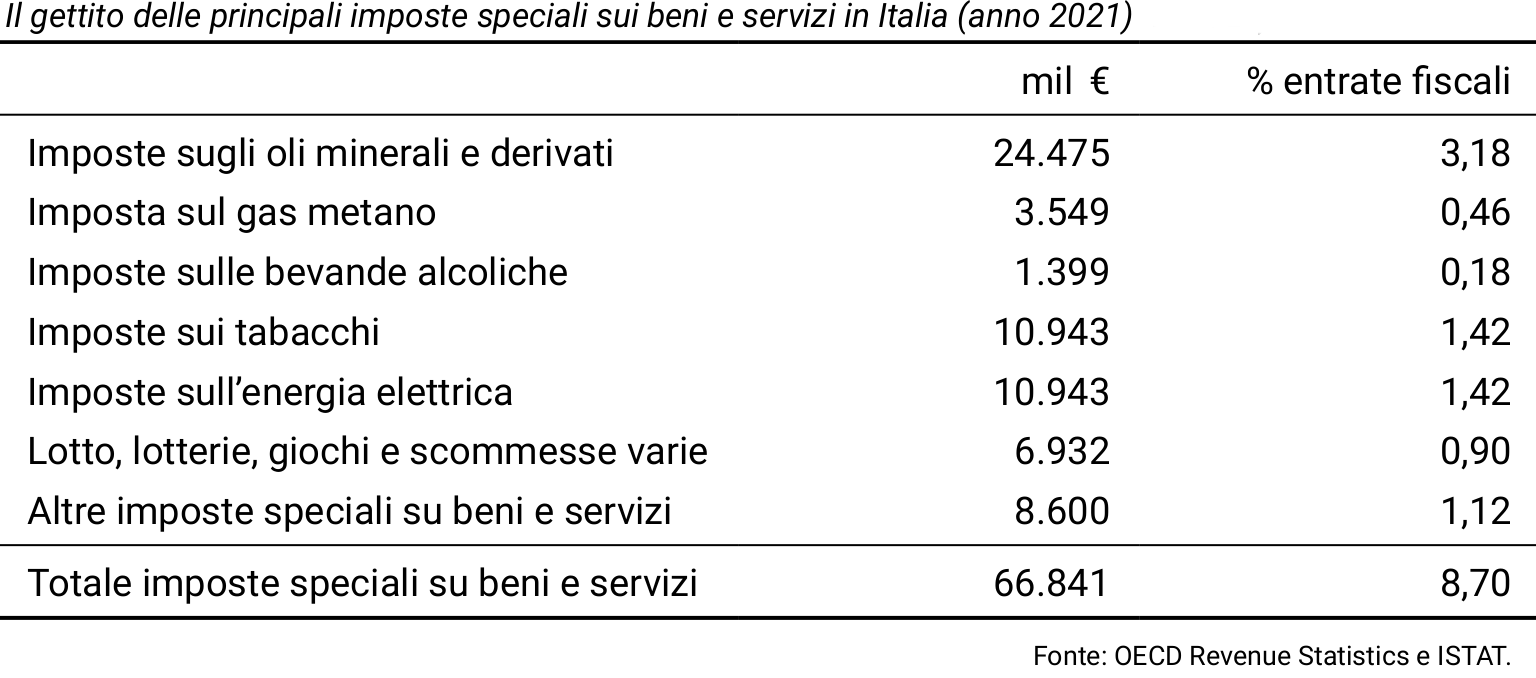
\includegraphics[width=\textwidth]{./figure/gettito-imposte-speciali-Italia-2021.png}
\end{center}
\end{frame}


\section{Il coordinamento internazionale}

%%%%%%%%%%%%%%%%%%%%%%%%%%%%%%%%%%%%%%%%%%%%
\begin{frame}{Problemi di coordinamento internazionale}

  \begin{itemize}
  \item \alert{Neutralità:} La imposte non dovrebbero distorcere i flussi
    commerciali e la concorrenza.
  \item \alert{Ripartizione del gettito tra paesi:} problemi di doppia
    imposizione, nel paese di origine e di destinazione della merce.
  \end{itemize}

  Al fine di evitare il problema della doppia tassazione, è possibile
  in linea di principio applicare uno dei seguenti due principi:
  \begin{block}{Principio di origine.} Il bene è assoggettato a Iva nel paese
    in cui è prodotto (paese esportatore), e non subisce tassazione al
    passaggio della frontiera
\end{block}
\begin{block}{Principio di destinazione.} L'imposta è applicata dal paese di
  destinazione, ove il bene è consumato.  All'esportazione il bene viene
  dunque "depurato" dell'Iva pagata fino a quel momento, mentre viene
  applicata l'Iva ai beni importati.  È il principio applicato in Europa.
\end{block}
\end{frame}

%%%%%%%%%%%%%%%%%%%%%%%%%%%%%%%%%%%%%%%%%%%%%%%%%%%
\begin{frame}{Il principio di destinazione}
  \begin{itemize}
  \item C'è consenso generale sulla preferibilità del principio di distinazione:
  \begin{itemize}
  \item (prescidendo da eventuali effetti dovuti alla traslazione
    dell'imposta) il gettito va interamente al Paese in cui il bene viene
    consumato, per cui ogni paese raccoglie il gettito a carico del
    consumatori residenti;
  \item il principio di destinazione garantisce che l'applicazione di imposte
    differenziate non influenzi i flussi di importazioni ed esportazioni.
  \end{itemize}
\item Nelle scelte del consumatore finale rileva il prezzo comprensivo di
  imposta:
  \begin{itemize}
  \item \(p =\) prezzo prima dell'imposta del bene prodotto nel paese;
  \item \(p^* =\) prezzo prima dell'imposta del bene prodotto all'estero.
  \end{itemize}
  \begin{equation*}
\begin{array}{cp{1.5cm}c}
   \text{(destinazione)} &&  \text{(origine)} \\
   \dfrac{q}{q^*}=\dfrac{p(1+\tau)}{p^*(1+\tau)}=\dfrac{p}{p^*} &&
   \dfrac{q}{q^*}=\dfrac{p(1+\tau)}{p^*(1+\tau^*)}\not= \dfrac{p}{p^*}.
\end{array}
\end{equation*}
\end{itemize}
\end{frame}

%%%%%%%%%%%%%%%%%%%%%%%%%%%%%%%%%%%%%%%%%%%%
\begin{frame}{Come si attua il principio di destinazione (in presenza di dogana)}

  \begin{itemize}
  \item L'imposta su applica sulle importazioni e non sulle esportazioni: le
    esportazioni sono operazioni \alert{non imponibili}.
  \end{itemize}

  \begin{figure}\centering
    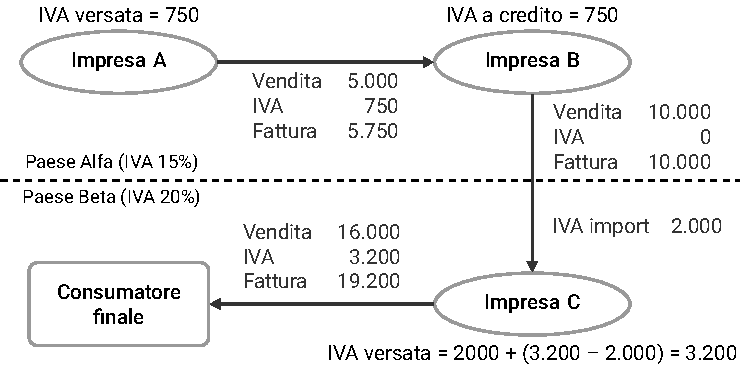
\includegraphics[width=.8\textwidth]{./figure/IVA-destinazione.pdf}
  \end{figure}

  \begin{itemize}
  \item L'Iva è versata interamente nel paese Beta, e il bene è gravato dalla
    relativa aliquota.
  \end{itemize}
\end{frame}

%%%%%%%%%%%%%%%%%%%%%%%%%%%%%%%%%%%%%%%%%%%%
\begin{frame}{Come si attua il principio di destinazione (in presenza di dogana) /2}

  \begin{itemize}
  \item Nel caso di \alert{importazioni destinate ai consumatori finali} del paese
    Beta l'imposta può essere riscossa al passaggio della dogana.
  \item Nel caso di \alert{acquisti diretti} di beni nel territorio nazionale da parte
    di non residenti l'applicazione del principio è più complessa. Nella UE:
    \begin{itemize}
    \item i residenti extra-UE possono chiedere un rimborso dell'IVA pagata
      per beni acquistati nella UE trasportabili nel proprio bagaglio
      personale;
    \item non è previsto il rimborso per l'IVA sui servizi;
    \item i residenti UE pagano comunque l'IVA del paese in cui hanno
      effettuato l'acquisto;
    \item per acquisti a distanza è prevista l'applicazione dell'IVA del paese
      di destinazione.
\end{itemize}
\end{itemize}
\end{frame}

%%%%%%%%%%%%%%%%%%%%%%%%%%%%%%%%%%%%%%%%%%%%
\begin{frame}{Il regime UE per gli scambi intracomunitari}

  \begin{itemize}
  \item Le importazioni intra-UE (\emph{acquisti intracomunitari}) hanno un
    trattamento diverso dalle importazioni da fuori UE, vista anche
    l'abolizione delle dogane nel 1993.
  \item Nel 1993, la proposta di assetto definitivo nel nuovo contesto di
    abolizione delle dogane prevedeva:
    \begin{itemize}
    \item passaggio al principio di origine con imponibilità delle
      esportazioni e non imponibilità delle importazioni;
    \item creazione di una \emph{stanza di compensazione} (\emph{clearing
        house}) per risolvere il problema della ripartizione del gettito;
    \item armonizzazione delle aliquote di imposta per evitare il rischio di
      concorrenza fiscale.
    \end{itemize}
  \item Nota bene: il sistema previsto, con il metodo imposta da imposta,
    avrebbe comunque garantito l'applicazione dell'aliquota del paese di
    destinazione nel caso delle transazioni B2B
  \end{itemize}
\end{frame}

%%%%%%%%%%%%%%%%%%%%%%%%%%%%%%%%%%%%%%%%%%%%
\begin{frame}{L'IVA in base all'origine nelle transazioni B2B}
\begin{figure}[htbp]
\centering
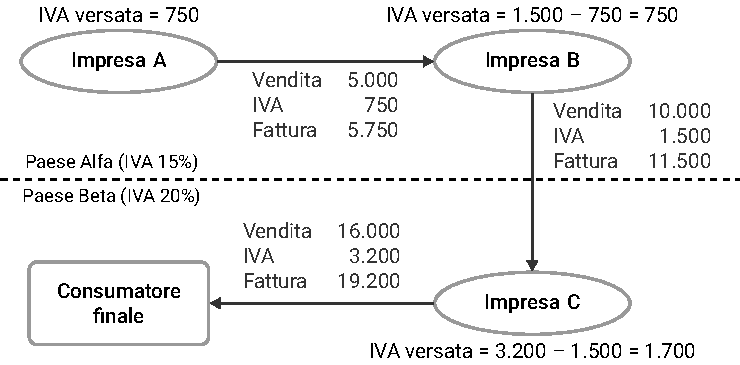
\includegraphics[width=.8\textwidth]{./figure/IVA-origine.pdf}
\end{figure}

\begin{itemize}
\item Il bene consumato in Beta è gravato dall'Iva di Beta: viene comunque
  garantita la neutralità;
\item il gettito non va interamente al paese dove ha luogo il consumo, ma
  viene ripartito tra i diversi paesi in proporzione al valore aggiunto.
\end{itemize}
\end{frame}

%%%%%%%%%%%%%%%%%%%%%%%%%%%%%%%%%%%%%%%%%%%%
\begin{frame}{Il regime «transitorio» vigente nella UE}
\begin{itemize}
\item La UE ha continuato ad adottare il \alert{regime transitorio} avviato nel 1993,
basato sul principio di \alert{destinazione}, ma adattato all'assenza di dogane:
\end{itemize}

\begin{figure}[htbp]
\centering
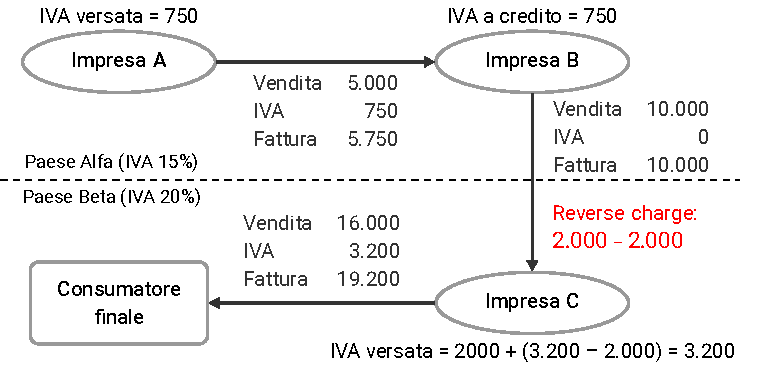
\includegraphics[width=.8\textwidth]{./figure/IVA-intracomunitaria.pdf}
\end{figure}

\footnotesize
L'impresa importatrice applica il \emph{reverse charge}: l'IVA sulle importazioni
non viene versata alla dogana (che non c'è!); l'impresa importatrice registra
IVA sul bene importato sia a debito che a credito (con aliquota del paese
destinazione); al momento della vendita del bene viene versata l'IVA con
l'aliquota del paese destinazione.
\end{frame}


%%%%%%%%%%%%%%%%%%%%%%%%%%%%%%%%%%%%%%%%%%%%
\begin{frame}{La nuova proposta di regime IVA nella UE}
\begin{itemize}
\item Orientamento più recente (2018): superamento del sistema vigente prevedendo
che l'impresa esportatrice applichi l'IVA con aliquota del paese
destinazione e il paese origine provveda a versare tale IVA al paese
destinazione.
\end{itemize}


\begin{figure}[htbp]
\centering
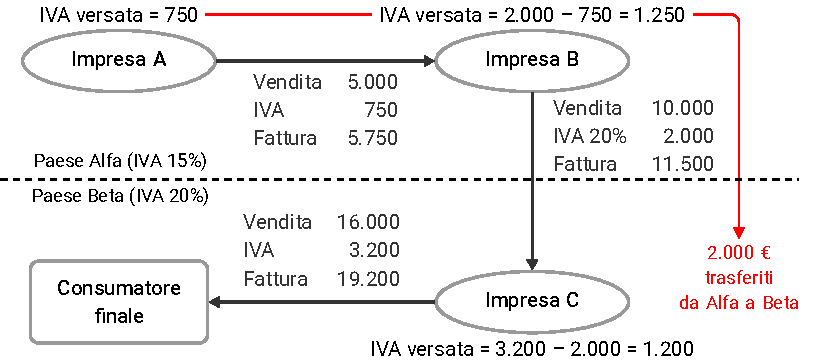
\includegraphics[width=.9\textwidth]{./figure/IVA-proposta-2018.pdf}
\end{figure}
\end{frame}
\end{document}


\end{document}